%% LyX 2.2.3 created this file.  For more info, see http://www.lyx.org/.
%% Do not edit unless you really know what you are doing.
\documentclass[11pt,twoside,english]{article}
\usepackage[T1]{fontenc}
%\usepackage[latin9]{inputenc}
\usepackage[a4paper]{geometry}
\geometry{verbose,tmargin=1in,bmargin=1in,lmargin=1.25in,rmargin=1.25in,headheight=1in,headsep=0.3in,footskip=0.8in}
\setcounter{tocdepth}{2}
\setlength{\parskip}{\bigskipamount}
\setlength{\parindent}{0pt}
\usepackage{babel}
\usepackage{float}
\usepackage{amsmath}
\usepackage{amsthm}
\usepackage{amssymb}
\usepackage{booktabs}
\usepackage[shortlabels]{enumitem}
\usepackage{graphicx,xspace}
\usepackage[unicode=true]{hyperref}
\usepackage[titletoc,title]{appendix}
% \usepackage{showframe} 
% \PassOptionsToPackage{unicode}{hyperref}

\makeatletter

%%%%%%%%%%%%%%%%%%%%%%%%%%%%%% LyX specific LaTeX commands.
%% Special footnote code from the package 'stblftnt.sty'
%% Author: Robin Fairbairns -- Last revised Dec 13 1996
\let\SF@@footnote\footnote
\def\footnote{\ifx\protect\@typeset@protect
    \expandafter\SF@@footnote
  \else
    \expandafter\SF@gobble@opt
  \fi
}
\expandafter\def\csname SF@gobble@opt \endcsname{\@ifnextchar[%]
  \SF@gobble@twobracket
  \@gobble
}
\edef\SF@gobble@opt{\noexpand\protect
  \expandafter\noexpand\csname SF@gobble@opt \endcsname}
\def\SF@gobble@twobracket[#1]#2{}
%% A simple dot to overcome graphicx limitations
\newcommand{\lyxdot}{.}

%% Self-defined macros
\newcommand{\Ap}{A\ensuremath{^\prime}\xspace}
\newcommand{\Bp}{B\ensuremath{^\prime}\xspace}

%%%%%%%%%%%%%%%%%%%%%%%%%%%%%% Textclass specific LaTeX commands.
\theoremstyle{plain}
\newtheorem{thm}{\protect\theoremname}[section]

\makeatother

\providecommand{\theoremname}{Theorem}

\begin{document}

\title{Designing Stable Coins}

\author{Yizhou CAO\thanks{\textit{Email}: \protect\href{mailto:yizhou.cao@finbook.co}{yizhou.cao@finbook.co},
CTO and Co-founder of FinBook}$\:,$ Min DAI\thanks{\textit{Email}: \protect\href{mailto:matdm@nus.edu.sg}{matdm@nus.edu.sg}. Director, Centre for Quantitative Finance, National University of Singapore}$\:,$ Steven KOU\thanks{\textit{Email}: \protect\href{mailto:matsteve@nus.edu.sg}{matsteve@nus.edu.sg}. Director, Risk Management Institute, National University of Singapore}$\:$, Lewei LI\thanks{\textit{Email}: \protect\href{mailto:lewei.li@finbook.co}{lewei.li@finbook.co}, CEO and Co-founder of FinBook}$\:$, Chen YANG\thanks{\textit{Email}: \protect\href{mailto:chen.yang@math.ethz.ch}{chen.yang@math.ethz.ch}, Department of Mathematics, ETH Zurich}}

%\date{}
\maketitle
\begin{abstract}

Stable coins, which are cryptocurrencies pegged to other stable financial assets, are desirable for blockchain networks to be used as public accounting ledgers for payment transactions  and as crypto money market accounts for asset allocation involving cryptocurrencies, whereby being often called the ``Holy Grail of cryptocurrency.'' However, existing cryptocurrencies, such as Bitcoins, are too volatile for these purposes. Inspired by the dual purpose funds popular in the US and China, we design, for the first time to our best knowledge, several dual-class structures that offer entitlements to either fixed income stable coins (class A funds) pegged to a traditional currency or leveraged investment opportunities (class B funds). Unlike traditional currencies, the new class A funds record all transactions on a blockchain without centralized counterparties. By using the option pricing theory, we show that proposed stable coins indeed have very low volatility, similar to that of the short term U.S. treasury bonds. When combined with insurance from a government, the design can also serve as a basis for issuing a sovereign cryptocurrency. 
\end{abstract}
\textit{Keywords:} stable coins, fixed income crypto asset, leveraged return crypto asset, smart contract, option pricing

\clearpage

\section{Introduction}
%\begin{flushright}
%{\small{}A wise man ought always to follow the paths beaten by great
%men, }\\
%{\small{}and to imitate those who have been supreme, so that }\\
%{\small{}if his ability does not equal theirs, at least it will savour
%of it.}\\
%{\small{}\textendash{} }\emph{\small{}Niccolo Machiavelli: The Prince}
%\par\end{flushright}{\small \par}


\subsection{Stablecoins and Fixed Income Assets}

Since their inception, crypto currencies aim to create an alternative financial system comparable to fiat financial systems. In a fiat system, money or credit exists in a few different forms: actual currency in circulation and fixed income assets such as time deposits and money market funds, which are the foundation for the rest of the financial market to build on. The crypto market is at primitive stage as it lacks coins or tokens comparable to fiat money due to their huge price volatility,  and thus there are no established fixed income assets either.

A Stable token, also known as stablecoin, is a crypto-token that keeps stable market value against a specific index, most noticeably US Dollar. There have been a few attempts to create stable tokens: Tether claims to have 1:1 USD collateral in its centralized bank accounts \cite{USDT}; Basecoin tries to control money supply by playing an algorithmic version of central bank \cite{Basecoin}; MakerDAO uses decentralized over-collateralization to maintain confidence of its Dai stablecoin \cite{MAKERDAO}.

Most stable token designs to date face a common problem: their holders bear variable levels of counter-party risks, but there is little incentive or even additional cost to hold these tokens. We believe a crypto-token with low price volatility and stable income is a superior safe haven asset and is essential for a more robust crypto market.

\subsection{Risk Segmentation}

In the fiat market, risk segmentation exists in every level of market. At asset class level, risk averse investors choose fixed income products while risk seeking investors choose equity or commodity. Within the fixed income market, conservative investors choose safe haven assets such as government bonds while aggressive players choose high yield bonds, or otherwise known as junk bonds.

Although most of crypto assets are considered highly speculative, there still exist different segments of risk appetites. The existence of margin trading in exchanges like BitFinex and Huobi Pro demonstrates the need of leverage from aggressive crypto investors. Similarly, safe haven assets providing low volatility and stable income will be appealing to institutional players, short-term pessimistic investors and ICO project teams. However, to our best knowledge, there is no viable product at the moment.

The price volatility cannot be eliminated, but can be transferred. Through a structured contract, a risk-seeking investor can get exposed to higher leverage with limited assets, while a risk-averse investor can avoid unwanted price fluctuations by entering the other side of the contract. The financial market has created many products satisfying different risk segments, some of which can be very practical for crypto market participants.

\subsection{Leveraged Funds}

Leverage is the strategy of using borrowed capital to increase the potential return of an investment \cite{Leverage}. Retail investors have less access to leverage methods such as margin loans and financial derivatives, which promotes the creation of leveraged fund products.

An interesting class of leveraged funds is the dual-purpose funds, also known as primes and scores, which are mutual funds that are split into two classes of shares by design: low risk shares and high risk shares. They were designed to provide investors with the opportunity of repackaging their investment incomes and capital flow in accordance with their preferences. Dual-purpose funds first appeared in U.S. in 1965, but faded out in early 1990s due to a change in the tax code that resulted in double taxation \cite{DM2018}. The valuation of dual-purpose funds in U.S. was investigated theoretically and empirically in \cite{Ingersoll1976} and \cite{JO}.

The dual-purpose fund was introduced in China in 2010 and it quickly became one of the most popular leveraged products there, reaching market size of 500 billion CNY (80 billion USD) at its peak. A Chinese dual-purpose fund usually takes an open-end index-tracking fund as underlying and has two classes of shares: the low risk A shares behave like a perpetual bond with periodical coupon payments, and the high risk B shares are essentially a closed-end fund magnifying the exposure of the underlying index. A set of upward and downward reset clauses is imposed to reduce the risk of both shares \cite{DM2018}.

We are inspired by the Chinese dual-purpose fund for three reasons: (i) both the income and leveraged shares answer unfulfilled demands of crypto-currency investors; (ii) the market mechanism, pricing formula, and arbitrage method prove to work in real market; and (iii) the structure can be efficiently implemented by Smart Contracts.

\subsection{Smart Contract}

Smart Contract was first proposed by Nick Szabo in 1994, who described it as \textquotedblleft a set of promises, specified in digital form, including protocols within which the parties perform on these promises\textquotedblright .

The idea has not received commercial adoption due to lack of trustworthy execution environment, until the appearance of blockchain technology. Released in 2015, Ethereum implements a nearly Turing-complete language on its blockchain, a prominent smart contract framework. The Ethereum white paper describes smart contracts as \textquotedblleft cryptographic boxes contain value and only unlock it if certain conditions are met". It also lists financial derivatives as the most common application of a smart contract, and introduces a rough idea about creating stable-value currencies through a hedging contract \cite{ETH}.

Up until now, the most popular stablecoin solution has been issuer-backed assets. And it is almost a market consensus that such issuers are not always trustworthy. We agree with Ethereum authors' argument that, a decentralized market of speculators and arbitragers powered by smart contract, could be an alternative solution.

This paper aims to propose an alternative approach of creating stable value tokens, providing a different set of trade offs between price stability, holder incentive and supply flexibility. We believe the solution will be very useful for broader adoption of the crypto market.

\clearpage{}

\section{Product Design\label{sec:Product-Design}}
%\begin{flushright}
%{\small{}Everything should be made as simple as possible, but no simpler.
%}\\
%{\small{}\textendash{} }\emph{\small{}Albert Einstein}
%\par\end{flushright}{\small \par}
In this section, we introduce the detailed design of our stable coin, including its creation/redemption, its cash flow, and related arbitrage mechanism. We also point out several differences between the product and the dual-purpose funds.

\subsection{Overview}

\paragraph{DUO }
a dual-class token structure that, combined with smart contract governed rules and market arbitrage mechanism, provides principal-guaranteed fixed incomes and leveraged capital gains for holders of each class, respectively.

\paragraph{Class A Token}
also known as the Income Token, continuously accumulates interests based on its original net value at last Reset event. It will also receive token payments at each Reset event.

\paragraph{Class B Token}
also known as the Leverage Token, entitles leveraged participation of the underlying digital assets.

The Custodian smart contract performs multiple tasks that facilitate key mechanism of the system, including: creation and redemption of DUO tokens, safekeeping the underlying digital assets (e.g. ETH), calculation of tokens' net values, and execution of Reset events.

\subsection{Creation and Redemption\label{subsec:Creation-and-Redemption}}

\subsubsection{Creation}

Dual-class tokens can be created by depositing underlying tokens to the Custodian contract. Upon receiving underlying tokens of amount $M_{C}$, the Custodian contract will return to the sender equal amount of Class A and Class B tokens. Such amount $C$ can be calculated by:
\begin{equation}
\begin{array}{c}
C=\frac{M_{C}\cdot P_{0}}{2}\ ,\end{array}\label{eq:creation}
\end{equation}
where $P_{0}$ is the recorded price of underlying token in USD at last reset event.

The deposited underlying tokens are kept by the Custodian contract, as collateral of the Class A and Class B tokens issued by the contract. Any user or member of the public can verify the collateral and tokens issued through third party applications such as \href{http://etherscan.io}{Etherscan.io}.

\subsubsection{Redemption}

Holders of Class A and Class B tokens can withdraw deposited underlying tokens at any time by performing a redemption. To do this, the user will send equal amount $C$ of Class A and Class B tokens to the Custodian contract. The contract will deduct Class A and Class B tokens, and return to the sender $M_{C}$ underlying tokens, where $M_{C}$ can be calculated by:
\begin{equation}
M_{C}=\frac{2C}{P_{0}}\ .\label{eq:redemption}
\end{equation}

\subsubsection{Net Value}

The net values of tokens are calculated based on the coupon rate, the elapsed time from last Reset event, and the latest underlying token price in USD fed to the system. In particular,
\begin{equation}
\begin{array}{ll}
V_{A}^{t}= & 1+R\cdot t,\\
V_{B}^{t}= & 2\cdot\frac{P_{t}}{P_{0}}-V_{A}^{t}\ ,
\end{array}\label{eq:netvalue}
\end{equation}
where $R$ is the \textbf{daily} coupon rate, $t$ is the number of days from last reset event, and $P_{t}$ is the current price of underlying token in USD.

\subsubsection{Implied Leverage Ratio}

Class B has the following leverage ratio:
$$
L_{B}^{t}  =\frac{P_{t}}{P_{0}}\cdot\frac{2}{V_{B}^{t}}.$$
Note that at inception or after resets, above simply reduces to $L_{B}^{0}=2$.

\subsection{Resets}

Simply put, the holders of Class B tokens borrow capital from the holders of Class A tokens and invest in a volatile asset (i.e. ETH), which leads the Class B token to possess a continuum of leverage ratios. To reduce risk of both classes, a set of upward and downward reset clauses is imposed. Resets preserve total value in the system.

\subsubsection{Contingent Upward Reset}

When underlying token price rises, the Class B token's leverage ratio reduces. An upward reset is triggered when the Net Value of Class B token reaches upper limit $\mathcal{H}_{u}$. The reset will restore the leverage ratio to 2. By increasing Class B's leverage ratio, the structure retains attraction to leverage-seeking users.

Upon upward reset:
\begin{enumerate}[1)]
\item Total amount of both classes token remains unchanged.
\item Net Value of both classes resets to 1 USD.
\item Both classes' holders will receive certain amount of underlying token from the Custodian contract. Such amount for each Class A token is
$\frac{V_{A}^{t-}-1}{P_{t}}$ and for each Class B token is $\frac{V_{B}^{t-}-1}{P_{t}}$
\end{enumerate}
Total value in the system is unchanged after reset. For details, see Appendix \ref{subsec:Contingent-Upward-Reset}.

\subsubsection{Contingent Downward Reset}

When the underlying token price falls, the Class B token's leverage ratio increases. A Downward Reset is triggered when the Net Value of Class B token reaches lower limit $\mathcal{H}_{d}$. Similar to an Upward Reset, a Downward Reset restores the leverage ratio. By reducing leverage ratio and restoring Net Value, the structure strengthens principal protection to Class A holders. Additionally, a Downward Reset will reduce the total supply of Class A and Class B tokens by roughly $1-\mathcal{H}_{d}$.

Upon downward reset:
\begin{enumerate}[1)]
\item Total amount of both classes token is reduced to $Q^{t+}=Q^{t-}\cdot V_{B}^{t-}$.
\item Net Value of both classes resets to 1 USD.
\item Class A holders will receive certain amount of underlying token from the Custodian contract. Such amount of each Class A token is: $\frac{V_{A}^{t-}-V_{B}^{t-}}{P_{t}}$
\end{enumerate}
Total value in the system is unchanged after reset. For details, see Appendix  \ref{subsec:Contingent-Downward-Reset}.

\subsubsection{Periodic Reset}

When a given time period $T$ has passed from the last reset time, or equivalently, $V_{A}^{t-}$ grows to upper limit $\mathcal{H}_{p}$, a periodic reset is triggered to restore the leverage ratio and net value of both classes. If $V_{B}^{t-}$ is less than 1, reset will be the same as the Contingent Downward reset. Otherwise, reset will be the same as the Contingent Upward reset.


\subsection{Market Mechanism}
% \begin{flushright}
% {\small{}Arbitrage human nature. It's not going to change any time
% soon. }\\
% {\small{}\textendash{} }\emph{\small{}James O'Shaughnessy}
% \par\end{flushright}{\small \par}

\subsubsection{Premium and Discount\label{subsec:Premium-and-Discount}}

Like all fixed income products, Class A is expected to trade on premium or at discount with respect to its net value, depending on market condition. When Class A trades on premium, that generally indicates a higher demand for income over leverage and thus Class A buyers are getting lower yield. On the contrary, when Class A trades at discount, that implies a higher demand for leverage over income and thus Class A buyers are paying less and getting higher yield. In an orderly market, Class A's market price can be used to derive the current market cost of funding. As net values draw closer to resets, Class A might trade closer to its net value as traders start exploiting arbitrage opportunities.

\subsubsection{Market Arbitrage }

The dual class tokens are two-way fungible to the underlying token (i.e. ETH). Thus, a price parity shall hold as below:
\[
P_{A}^{t}+P_{B}^{t}=V_{A}^{t}+V_{B}^{t}\ ,
\]
where $P_{A}^{t}$ is the current price of Class A in USD, and $P_{B}^{t}$ is the current price of Class B in USD.

Along with Equation (\ref{eq:netvalue}) in Section \ref{subsec:Creation-and-Redemption}, the following relation should hold:
\[
P_{A}^{t}+P_{B}^{t}=2\cdot\frac{P_{t}}{P_{0}}\ .
\]
On open market, arbitrage opportunity exists when Class A and Class B tokens trade away from their net values and the above equation is likely violated on either side.

\paragraph{Arbitrage via Creation}

When combined market price of Class A and Class B tokens are higher than their combined net values, i.e.
\[
P_{A}^{t}+P_{B}^{t}>2\cdot\frac{P_{t}}{P_{0}}\ ,
\]
arbitrage profit can be exploited by perform DUO token creation:
\begin{enumerate}[1)]
\item Buy 1 underlying tokens from open market for $P_{t}$ USD equivalent.
\item Send the underlying tokens to the Custodian contract.
\item Based on Equation (\ref{eq:creation}), receive $\frac{P_{0}}{2}$ Class A and $\frac{P_{0}}{2}$ Class B tokens.
\item Sell Class A and Class B tokens on open market for $P_{0}\cdot\frac{P_{A}^{t}+P_{B}^{t}}{2}$ USD equivalent.
\end{enumerate}
The expected payoff of above operations is:
\[
P_{0}\cdot\frac{P_{A}^{t}+P_{B}^{t}}{2}-P_{t}=\frac{P_{0}}{2}\cdot\left(P_{A}^{t}+P_{B}^{t}-2\cdot\frac{P_{t}}{P_{0}}\right)>0\ .
\]

\paragraph{Arbitrage via Redemption}

When combined market price of Class A and Class B tokens are lower than their combined net values, i.e.
\[
P_{A}^{t}+P_{B}^{t}<2\cdot\frac{P_{t}}{P_{0}}\ ,
\]
arbitrage profit can be exploited by perform DUO token redemption:
\begin{enumerate}[1)]
\item Buy $\frac{P_{0}}{2}$ Class A and $\frac{P_{0}}{2}$ Class B tokens from open market for $P_{0}\cdot\frac{P_{A}^{t}+P_{B}^{t}}{2}$ USD equivalent.
\item Send Class A and Class B tokens to the Custodian contract.
\item Based on Equation (\ref{eq:redemption}), receive 1 underlying tokens.
\item Sell underlying tokens on open market for $P_{t}$ USD equivalent.
\end{enumerate}
The expected payoff of above operations is:
\[
P_{t}-P_{0}\cdot\frac{P_{A}^{t}+P_{B}^{t}}{2}=\frac{P_{0}}{2}\cdot\left(2\cdot\frac{P_{t}}{P_{0}}-\left(P_{A}^{t}+P_{B}^{t}\right)\right)>0\ .
\]
Many other factors also determine whether above arbitrage strategy can be successfully executed, such as bid ask spread of all the 3 components, cost in creation and redemption, and ability to short sell the required components. Please refer to appendix for discussion of a more general case.


\subsection{Differences from the Dual-Purpose Fund Contract}
Although the contract of DUO is inspired by dual-purpose funds, it is different from dual-purpose funds in U.S. and China in the aspects shown in Table \ref{tbl:difference}.

\begin{table}[h]
	\caption{Contract Comparison of DUO and Dual-Purpose Fund in U.S. and China}\label{tbl:difference}
	\vspace{1em}
	\scriptsize
	\begin{tabular}{@{}c c c c c c@{}}
	\toprule
		& \begin{tabular}{@{}c@{}}Payment Style\\ of A Share\end{tabular} & \begin{tabular}{@{}c@{}}Payment Style\\ of B Share\end{tabular} & \begin{tabular}{@{}c@{}}Leverage Ratio\\ Reset\end{tabular} & Lifespan & \begin{tabular}{@{}c@{}}Reference Asset\end{tabular} \\ \midrule
	\begin{tabular}{@{}c@{}}Dual-Purpose\\ Fund in U.S.\end{tabular} & Dividend & \begin{tabular}{@{}c@{}}Single payment\\ at wind-up date\end{tabular}  & No & Finite & Stock/ Stock Index\\ \midrule
	\begin{tabular}{@{}c@{}}Dual-Purpose\\ Fund in China\end{tabular} & Fixed Income &  \begin{tabular}{@{}c@{}}Periodic payments\\ at upward reset dates\end{tabular} & Yes & Infinite & Stock Index\\ \midrule
	DUO & Fixed Income & \begin{tabular}{@{}c@{}}Periodic payments\\at all reset dates\end{tabular} & Yes & Infinite & \begin{tabular}{@{}c@{}}USD denominated\\ crypto-currency value\end{tabular}\\
	\bottomrule
	\end{tabular}
	\par\flushleft\scriptsize The dual-purpose funds in U.S. include those studied in \cite{Ingersoll1976} and the prime and scores studied in \cite{JO}.
\end{table}

There is one more (technical) difference between DUO with dual-purpose funds in China. For the dual-purpose funds, the upward reset is triggered by the underlying up-crossing $\mathcal{H}_u$ while the downward reset is triggered by the Net Value of B share down-crossing $\mathcal{H}_d$. In contrast, for DUO, the triggering conditions of both upward and downward resets are all based on the Net Value of Class B token. This brings about symmetry and simplicity to the triggering condition, making it easier to understand.

Both the dual-purpose funds and DUO values can be characterized in terms of partial differential equation (PDE). However, their PDEs differ in the following aspects.
\begin{table}[h]
	\caption{Model Comparison of DUO and Dual-Purpose Fund in U.S. and China}\label{tbl:modeldiff}
	\vspace{1em}
	\scriptsize
	\begin{tabular}{@{}c c c@{}}
	\toprule
		& Pricing Method & Domain of PDE\\ \midrule
		\begin{tabular}{@{}c@{}}Dual-Purpose\\ Fund in U.S.\end{tabular} & Black-Scholes PDE & Half bounded ($S>0$) \\ \midrule
		\begin{tabular}{@{}c@{}}Dual-Purpose\\ Fund in China\end{tabular} & \begin{tabular}{@{}c@{}} Periodic PDE with nonlocal terminal\\ and boundary conditions\end{tabular} & \begin{tabular}{@{}c@{}}Bounded, with time-dependent lower bound\\ and time-independent upper bound\end{tabular}\\ \midrule
		DUO & \begin{tabular}{@{}c@{}} Periodic PDE with nonlocal terminal\\ and boundary conditions\end{tabular} & \begin{tabular}{@{}c@{}}Bounded, with time-dependent\\ lower and upper bound\end{tabular}\\
	\bottomrule
	\end{tabular}
\end{table}

\clearpage

\section{Valuation}\label{sect:valuation}

Denote $W_{A}$ and $W_{B}$ as the market value of Class A and Class B, respectively. Denote $S_t=P_t/P_0$ as the relative price of the underlying token. By the design of contract, $S$ returns to 1 at every reset date.

Under the risk-neutral pricing framework, the current market value of Class A token is given recursively as
\begin{align}
\begin{split}W_{A}(t,S) & =E_{t}\Bigg[e^{-r(\zeta-t)}[RT+g(S_{\zeta-})+(1-g(S_{\zeta-}))W_{A}(0,1)]\cdot\mathbf{1}_{\{\zeta\le\tau,\eta\}}\\
 & \quad+e^{-r(\tau-t)}(R\tau+W_{A}(0,1))\cdot\mathbf{1}_{\{\tau<\eta,\zeta\}}\\
 & \quad+e^{-r(\eta-t)}(R\eta+1-V_{B}^{\eta-}+V_{B}^{\eta-}W_{A}(0,1))\cdot\mathbf{1}_{\{\eta<\tau,\zeta\}}\Bigg],
\end{split}
\label{VAL2}
\end{align}
where $E_{t}$ is the expectation computed under the risk-neutral measure and under the initial condition $S_{t-}=S$, random times $\zeta$, $\tau$ and $\eta$ represent the first periodic, upward and downward reset date from $t$, respectively, and $g(s)=((1+\alpha)(1-s)+\alpha RT)^{+}$. $W_{A}(t,S)$ denotes the market value of Class A token with time from last interest payment $0\le t\le1$, with $H_{d}(t)\le S\le H_{u}(t)$ and $0\le t<T$, where $H_{d}(t)=\frac{\alpha}{1+\alpha}(1+Rt)+\frac{1}{1+\alpha}\mathcal{H}_{d}$, and $H_{u}(t)=\frac{\alpha}{1+\alpha}(1+Rt)+\frac{1}{1+\alpha}\mathcal{H}_{u}$. Once we calculate $W_A$, the value of Class B token can be calculated as $W_B=(1+\alpha)S-\alpha W_A$.

The value of Class A can be determined as above in a recursive manner, since investors still get Class A token in addition to the payments after a reset. On the right hand side, the second and third terms describe the cash flow on upward and downward resets. The second term shows that, if the reset is an upward reset, investors get coupon payment, and the time from last reset changes to 0 and $S$ to $1$. The third term shows that, if a downward reset comes first, investors receive payment of value $V_{A}^{\eta-}-V_{B}^{\eta-}$ (including coupon payment of value $V_{A}^{\eta-}-1$ and compensation for the quantity reduction $1-V_{B}^{\eta-}$), each Class A token reduces to $V_{B}^{\eta-}$ token, and the time from last reset changes to 0 and $S$ to $1$. Finally, the first term is value of the cash flow on the periodic reset date. Specifically, when $V_{B}^{\zeta-}\ge1$, or equivalently, $(1+\alpha)-\alpha(1+RT)\ge1$ (so that $g(S_{\zeta-})=0$), the cash flow follows that of an upward reset where Class A receives payment of value $RT$, and the number of Class A remains unchanged; when $V_{B}^{\zeta-}<1$, or equivalently, $(1+\alpha)-\alpha(1+RT)<1$, the cash flow follows that of a downward reset, where Class A receives coupon and compensation payment of value $V_{A}^{\zeta-}-V_{B}^{\zeta-}=1+RT-(1+\alpha)S_{\zeta-}-\alpha(1+RT)=RT+g(S_{\zeta-})$, and each token of Class A is reduced to $V_{B}^{\zeta-}=(1+\alpha)S_{\zeta-}-\alpha(1+RT)=1-g(S_{\zeta-})$ token.

One can estimate $W_A$ via \eqref{VAL2} using Monte Carlo simulation, which is also proposed by \cite{AC} to deal with the complexities in the fund contract. Due to the high volatility of the underlying token price, it is important to achieve real-time calculation of $W_A$. However, the efficiency of the simulation-based method is not high enough for this purpose, since the cash flow of Class A token has an infinite horizon and a weakly path-dependent nature. Therefore, in the following we propose an efficient PDE-based estimation method.

We assume that $P$ follows a geometric Brownian motion under the risk neutral measure:
\begin{align*}
dP_{t}=r Pdt+\sigma P_{t}dW_{t},
\end{align*}
where $W_{t}$ is a one-dimensional standard Brownian motion. Then, $W_{A}$ can be characterized in terms of a partial
differential equation:

\begin{align}\label{eqn:PDEstart}
-\frac{\partial W_{A}}{\partial t} & =\frac{1}{2}\sigma^{2}S^{2}\frac{\partial^{2}W_{A}}{\partial S^{2}}+r S\frac{\partial W_{A}}{\partial S}-r W_{A}, ~~t\in[0,T),~S\in (H_d(t),H_u(t))\\\label{eqn:ter}
W_{A}(T,S) & =RT+g(S)+(1-g(S))W_{A}(0,1),\\\label{eqn:bound1}
W_{A}(t,H_{u}(t)) & =Rt+W_{A}(0,1)\\\label{eqn:PDEend}
W_{A}(t,H_d(t)) & =Rt+1-\mathcal{H}_{d}+\mathcal{H}_{d}W_{A}(0,1).
\end{align}

The main feature of the above PDE problem is the nonlocal terminal and boundary conditions $\eqref{eqn:ter}$ \textendash{} $\eqref{eqn:PDEend}$, where the given data also depend on the solution $W_{A}$ itself. Although $\eqref{eqn:PDEstart}$ involves the standard Black-Scholes operator (due to our geometric Brownian motion assumption), the presence of the solution $W_{A}$ in terminal and boundary data makes the PDE significantly different from the classical Black-Scholes PDE, leading to challenges in both theoretical and numerical aspects. On the theoretical aspect, the existing stochastic representation result is not applicable to PDE $\eqref{eqn:ter}$ \textendash{} $\eqref{eqn:PDEend}$ due to the nonlocalness of the terminal and boundary conditions. On the numerical aspect, the nonlocalness in the terminal and boundary data also causes problem since a numerical solution in the interior region depends on the boundary and terminal data, which in turns depends on the numerical solution in the interior region. To solve this, we propose an iterative procedure presented in Appendix $\ref{subsec:Numerical-Procedure-for}$.

The nonlocal terminal and boundary conditions in $\eqref{eqn:ter}$ \textendash{} $\eqref{eqn:PDEend}$ are directly related with the cash flow of Class A token. The upper boundary condition ($\ref{eqn:bound1}$) at $S=H_{u}(t)$ corresponds to the upward reset, when early payment $Rt$ is delivered and $S$ resets to 1; the lower boundary condition ($\ref{eqn:PDEend}$) at $S=H_d(t)$ corresponds downward reset, when early payment $V_{B}-V_{A}$ is delivered, each Class A token shrinks to $\mathcal{H}_{d}$ token, and $S$ resets to 1.\footnote{Since $P$ has continuous sample path due to the geometric Brownian motion assumption, we have $V_B^{\eta-}=\mathcal{H}_d$ on downward resets.} Finally, the terminal condition ($\ref{eqn:ter}$) corresponds to the periodic reset, where the payment follows either the upward or downward reset based on whether $V_{B}\le1$.


\clearpage

\section{Extensions}
To make the stable token defined in Section \ref{sec:Product-Design} even more stable, we consider two extensions on the DUO contract, which split Class A token into two further classes of token.

\subsection{A=A0+A1}
This extension splits Class A further into two sub-classes: A0 and A1. At the creation of DUO, each Class A token is split into one Class A0 token and one Class A1 token. On the next reset date $t$, Class A1 receives the coupon payment $V_A^{t-}-1$ for Class A, and then Class A1 is terminated. Class A0 receives ETH token with value $(1-V_B^{t-})^+$ as liquidation payment, and is then split into $1-(1-V_B^{t-})^+$ Class A0 token and $1-(1-V_B^{t-})^+$ Class A1 token, until the next reset when Class A1 receives payment and A0 is split again, so on and so forth.\footnote{Note that when $V_B^{t-}\ge 1$, Class A0 does not receive any underlying token and maintains the same quantity.} At any time, the quantity of Class A0 and A1 maintains 1:1. Based on this construction, at any time, the value of Class A1 equals the expected discounted value of Class A's next payment on the next reset date, and the value of Class A0 equals the difference between values of Class A and A1, or the expected present value of all future payments except the first one.

By contract design, the coupon of Class A1 is delivered in the form of the underlying token, whose value in USD may subject to volatile changes due to the high volatility of ETH. In contrast, the coupon of Class A0 is paid in the form of Class A1 token, whose value in USD is much less volatile compared to ETH. Therefore, Class A0 is more suitable for investors with lower risk tolerance or are less active on the market; upon receiving Class A1 tokens as coupon, they have a relatively longer period of time to liquidate the token before its value changes noticeably. In contrast, Class A1 is more suitable for investors who are willing to take certain degree of risk and are more active on the market; so that upon receiving the underlying token, they can monitor the market actively and spot a good opportunity to liquidate the underlying token.

Under the risk-neutral pricing framework, the market value of Class A1 token is given recursively as
\begin{align*}
W_{A}(t,S) & =E_{t}\Bigg[e^{-r(\zeta-t)}RT\cdot\mathbf{1}_{\{\zeta\le\tau,\eta\}}+e^{-r(\tau-t)}R\tau\cdot\mathbf{1}_{\{\tau<\eta,\zeta\}}+e^{-r(\eta-t)}R\eta\cdot\mathbf{1}_{\{\eta<\tau,\zeta\}}\Bigg],
\end{align*}
where the first periodic reset time $\zeta$, the first upward reset time $\tau$ and the first downward reset time $\eta$ are defined in the same way as \eqref{VAL2}.  $W_{A1}$ corresponds to the following PDE
\begin{align*}
-\frac{\partial W_{A1}}{\partial t} & =\frac{1}{2}\sigma^{2}S^{2}\frac{\partial^{2}W_{A1}}{\partial S^{2}}+r S\frac{\partial W_{A1}}{\partial S}-r W_{A1},~~t\in[0,T),~S\in (H_d(t),H_u(t))\\
W_{A1}(T,S) & =RT\\
W_{A1}(t,H_{u}(t)) & =Rt\\
W_{A1}(t,H_d(t)) & =Rt.
\end{align*}
Finally, the value of Class A0 token is defined as $W_{A0}=W_A-W_{A1}$.

\subsection{\texorpdfstring{A=\Ap+\Bp}{Lg}}
This second extension splits Class A into two sub-classes: Class \Ap and \Bp. Class \Ap and \Bp invest in Class A token. At any time, a quantity of $\frac{2}{\bar{P}_A}$ Class A token can be split into one Class \Ap and one Class \Bp token, where $\bar{P}_A=W_A(0,1)$. Conversely, one Class \Ap and \Bp token can be merged into $\frac{2}{\bar{P}_A}$ Class A token. The net asset value of Class \Ap is defined as $V_{A^\prime}=1+R^\prime t$, where $t$ is the time since last reset, and the net asset value of Class \Bp is defined as $V_{\Bp}=\frac{2W_A}{\bar{P}_A} - V_{A^\prime}$, where $W_A$ is the price of Class A.

Class A$^\prime$ and B$^\prime$ reset \emph{when and only when} Class A resets. All payments to Class \Ap and \Bp (in the form of underlying token) consist of the payments made to the Class A in which \Ap and \Bp invest. Specifically,
\begin{itemize}
	\item On periodic reset $\zeta$, Class \Ap and \Bp receive $R^\prime T + g(S_{\zeta-})$ and $2RT-R^\prime T+ g(S_{\zeta-})$, respectively, in the form of underlying token, and each one Class A$^\prime$ and B$^\prime$ becomes $1-g(S_{\zeta-})$ share (if $g(S_{\zeta-})=0$, then no compensation and reduction in share quantity);
	\item On upward reset $\tau$, Class \Ap and \Bp receive payment with value $R^\prime t$ and $2Rt-R^\prime t$, respectively, in the form of underlying token;
	\item On downward reset $\eta$, Class A$^\prime$ and Class \Bp receive $R^\prime t + 1-V_B^{\eta-}$ and $2Rt-R^\prime t+ 1-V_B^{\eta-}$, respectively, in the forms of underlying token, and each one Class A$^\prime$ and B$^\prime$ becomes $V_B^{\eta-}$ share.
\end{itemize}

When Class \Ap and Class A have the same coupon rate, i.e. $R^\prime=R$, then Class A, \Ap and \Bp have the same cash flow and hence the same value, provided no extreme event occurs (the net asset value of Class B does not jump to a negative level). In practice, $R^\prime$ is typically smaller than $R$ and close to the risk-free rate. For instance, $R^\prime = 0.03$ p.a.

Under the risk-neutral pricing framework, the value of Class \Ap is given as
\begin{align}
\begin{split}W_{A^\prime}(t,S) & =E_{t}\Bigg[e^{-r(\zeta-t)}[R^\prime T+g(S_{\zeta-})+(1-g(S_{\zeta-}))W_{A^\prime}(0,1)]\cdot\mathbf{1}_{\{\zeta\le\tau,\eta\}}\\
 & \quad+e^{-r(\tau-t)}(R^\prime\tau+W_{A^\prime}(0,1))\cdot\mathbf{1}_{\{\tau<\eta,\zeta\}}\\
 & \quad+e^{-r(\eta-t)}(R^\prime\eta+1-V_{B}^{\eta-}+V_{B}^{\eta-}W_{A^\prime}(0,1))\cdot\mathbf{1}_{\{\eta<\tau,\zeta\}}\Bigg],
\end{split}
\end{align}
where $\zeta,\tau,\eta$ are the first periodic, upward or downward reset (whichever comes first) of Class A (or equivalently, Class \Ap and \Bp) after $t$, respectively. 

$W_{A^\prime}$ satisfies the following PDE, which is the same to \eqref{eqn:PDEstart} -- \eqref{eqn:PDEend} except for changing $R$ to $R^\prime$:
\begin{align*}
-\frac{\partial W_{A^\prime}}{\partial t} & =\frac{1}{2}\sigma^{2}S^{2}\frac{\partial^{2}W_{A^\prime}}{\partial S^{2}}+r S\frac{\partial W_{A^\prime}}{\partial S}-r W_{A^\prime}, ~~t\in[0,T),~S\in (H_d(t),H_u(t))\\
W_{A^\prime}(T,S) & =R^\prime T+g(S)+(1-g(S))W_{A^\prime}(0,1),\\
W_{A^\prime}(t,H_{u}(t)) & =R^\prime t+W_{A^\prime}(0,1)\\
W_{A^\prime}(t,H_d(t)) & =R^\prime t+1-\mathcal{H}_{d}+\mathcal{H}_{d}W_{A^\prime}(0,1).
\end{align*}

Given $W_{\Ap}$, the value of Class \Bp is given as $\frac{2W_A(t,S)}{W_A(0,1)}-W_{\Ap}$.

Although Class \Ap and A look similar under normal situations, under extreme scenario in practice, Class \Ap is safer than Class A. Consider the scenario when the underlying value suddenly drops to a level $P_t<\frac{P_0}{2}(1+Rt)$. In this case, the net asset value of Class B, $V_B$, becomes negative. A downward reset will be triggered, when Class A gets all the remaining value $\frac{2P_t}{P_0}$, Class B gets nothing, and all Class A and B tokens are liquidated. This means that Class A will suffer a loss (getting a liquidation value $\frac{2P_t}{P_0}$ smaller than its net asset value $1+Rt$) if $P_t$ suddenly drops below $P_t<\frac{P_0}{2}(1+Rt)$. In comparison, under the same scenario, Class \Ap and \Bp will get $\frac{4P_t}{P_0}$ in the form of underlying token from Class A. Therefore, Class \Ap will have a loss if and only if $\frac{4P_t}{P_0}<1+R^\prime t$, or equivalently, $P_t<\frac{P_0}{4}(1+R^\prime t)$, and when $\frac{P_0}{4}(1+R^\prime t)<P_t<\frac{P_0}{2}(1+Rt)$, Class \Ap will get full payment $1+R^\prime t$ while Class A will have a loss.

\clearpage

\section{ETH Examples}

For illustration, we hereby uses Ether (ETH) as the underlying token
and apply below parameter values:
\begin{align*}
R& =0.02\% & R^\prime & = 0.0082\% \text{ (3\% p.a.)}\\
\mathcal{H}_{u} & =2 & \mathcal{H}_{p} & =1.02\\
\mathcal{H}_{d} & =0.25 & \alpha &=1\\
T &= 100/365. & r&=0.0082\% \text{ (3\% p.a.)}.
\end{align*}
Note that the choice of $T$ means that the length of reset period equals $N=100$ days.
The following assumptions are used:
\begin{enumerate}
\item Price is monitored on \textbf{daily} basis
\item Resets are performed according to end-of-day prices
\item The structure starts with 100,000 ETH with no further capital injection
\item Reinvestment of ETH payout from resets is not considered
\end{enumerate}

\subsection{Overall Market}

ETH/USD price data from 1 Oct 2017 to 28 Feb 2018 is used. In this period, ETH started from 303.95 USD to low of 284.92 USD and high of 1,359.48 and ended at 851.5.

At inception, 15,197,500 Class A and 15,197,500 Class B are issued from the 100,000 ETH, total value in the system is 30,395,000 USD.

Three upward resets were triggered on 24 Nov 2017 ($V_{B}=2.0846$), 17 Dec 2017 ($V_{B}=2.0467$) and 7 Jan 2018 ($V_{B}=2.1106$) while one downward reset was triggered on 5 Feb 2018 ($V_{B}=0.2379$.). No periodic reset was triggered in the sampling period.\\

\begin{figure}[H]
\begin{centering}
\includegraphics[scale=0.9]{2\lyxdot 4_TotalValue}
\par\end{centering}
\caption{Total Values}

\end{figure}

\begin{figure}[H]
\begin{centering}
\includegraphics[scale=0.9]{2\lyxdot 4_NetValue}
\par\end{centering}
\caption{Net Values}
\end{figure}

\paragraph{Period without Reset}

The total value of Class A and Class B tokens moves in line with ETH price. Class B tokens get exposed to full price fluctuations of ETH, while Class A token value is stable and slowly appreciating.\\

\begin{figure}[H]
\begin{centering}
\includegraphics[scale=0.9]{2\lyxdot 4_No_Reset_TotalValue}
\par\end{centering}
\caption{1 Oct 2017 - 23 Nov 2017 Total Values}
\end{figure}

\paragraph{Period with Contingent Upward Reset\protect\footnote{Chart and numbers are similar for the other two upward resets and thus omitted here.}}

17 Dec 2017, $V_{B}=2.0467$. 97.4049 ETH is paid out to Class A holders and 22,163.7213 ETH is paid out to Class B holders. Remaining System value is at 30,395,000 USD. The total value of Class A, Class B and ETH payout is consistent with ETH price movement.\\

\begin{figure}[H]
\begin{centering}
\includegraphics[scale=0.9]{2\lyxdot 4_Upward_TotalValue}
\par\end{centering}
\caption{24 Nov 2017 - 6 Jan 2017 Total Values}
\end{figure}

\paragraph{Period with Contingent Downward Reset}

5 Feb 2018, $V_{B}=0.2379$. 16,789.3847 ETH is paid out to Class A holders. total amount of both classes is reduced to 3,615,680.02. Remaining System value is at 7,231,360.04 USD. The total value of Class A, Class B and ETH payout is consistent with ETH price movement.\\

\begin{figure}[H]
\begin{centering}
\includegraphics[scale=0.9]{2\lyxdot 4_Downward_TotalValue}
\par\end{centering}
\caption{7 Jan Nov 2017 - 28 Feb 2017 Total Values}
\end{figure}

\subsection{Individual Class Return}

\paragraph{Class A}

stable return from daily coupon and not affected by ETH price movement.\\

\begin{figure}[H]
\begin{centering}
\includegraphics[scale=0.9]{2\lyxdot 4_A_Return}
\par\end{centering}
\caption{Class A Return}
\end{figure}

\paragraph{Class B}

magnified return from ETH price movement due to the embedded leverage.\\

\begin{figure}[H]
\begin{centering}
\includegraphics[scale=0.9]{2\lyxdot 4_B_Return}
\par\end{centering}
\caption{Class B Return}
\end{figure}

\paragraph{Note}

In order to achieve above return, ETH payout from resets need to be fully converted back to the corresponding class token. For example, after 24 Nov 2017 upward reset, all ETH received by Class A holder need to be converted into Class A token.

\subsection{Market Value of Class A and Class B}

\begin{figure}[H]
\begin{centering}
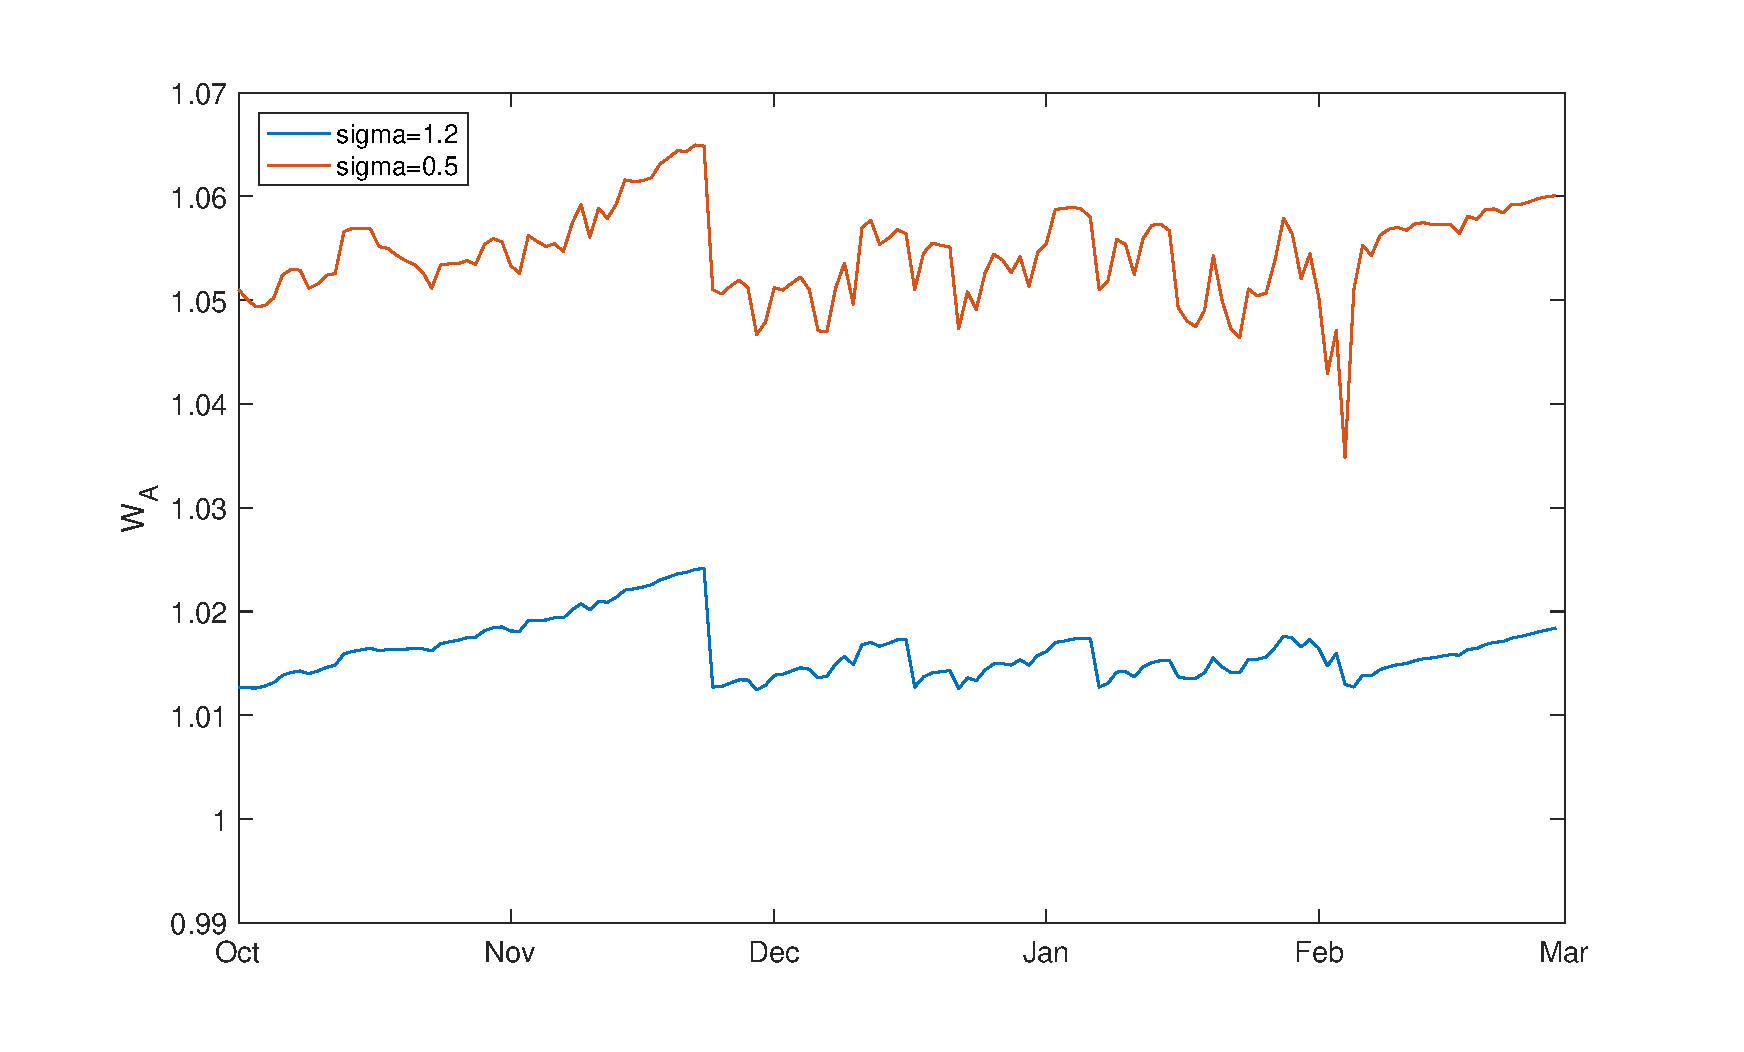
\includegraphics[width=0.95\textwidth]{WA.eps}
\par\end{centering}
\caption{Class A Market Value. Parameters: $R=0.02\%,\mathcal{H}_{d}=0.25,\mathcal{H}_{u} =2,\mathcal{H}_{p}=1.02,N=100,\alpha=1$.}\label{fig:valA}
\end{figure}

Figure \ref{fig:valA} shows that, although Class A has a fixed coupon rate, and its coupon payment is periodic and protected by the resets, its value is still volatile on non-coupon dates. This behavior is similar to a junk bond, whose value is influenced by its issuer's credit risk. In contrast, the main risk of Class A is not credit risk, but the risk of a downward reset. On a downward reset, a portion of Class A token will be liquidated, so the investor will lose the value of future coupons that would be generated from this portion. Therefore, an approaching downward reset will pull down the value of Class A. This is illustrated in Figure \ref{fig:valA} at the end of January: as the downward reset approaches, the value of Class A also goes down, especially when the model underestimates the market volatility (by setting $\sigma=0.5$).


\begin{figure}[H]
\begin{centering}
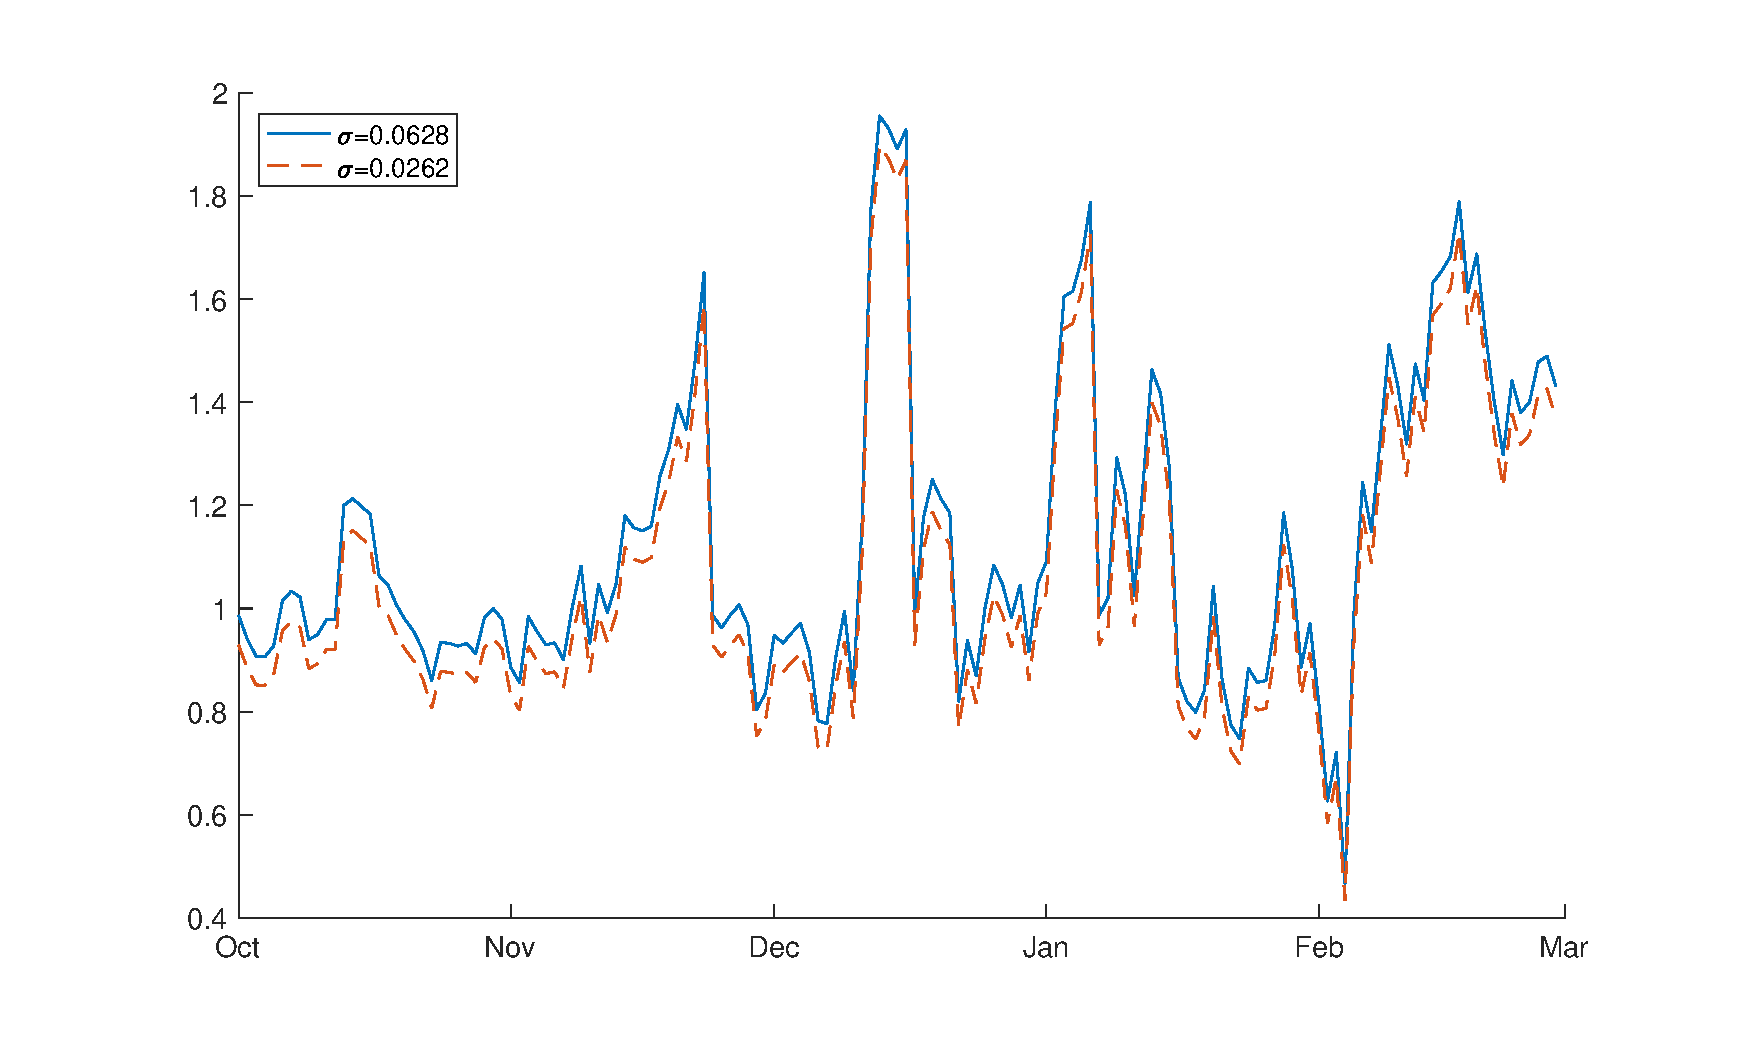
\includegraphics[width=0.95\textwidth]{WB}
\par\end{centering}
\caption{Class B Market Value. Parameters: $R=0.02\%,\mathcal{H}_{d}=0.25,\mathcal{H}_{u} =2,\mathcal{H}_{p}=1.02,N=100,\alpha=1$.}
\end{figure}


\subsection{Market Value of Class A0}
\begin{figure}[H]
\centering
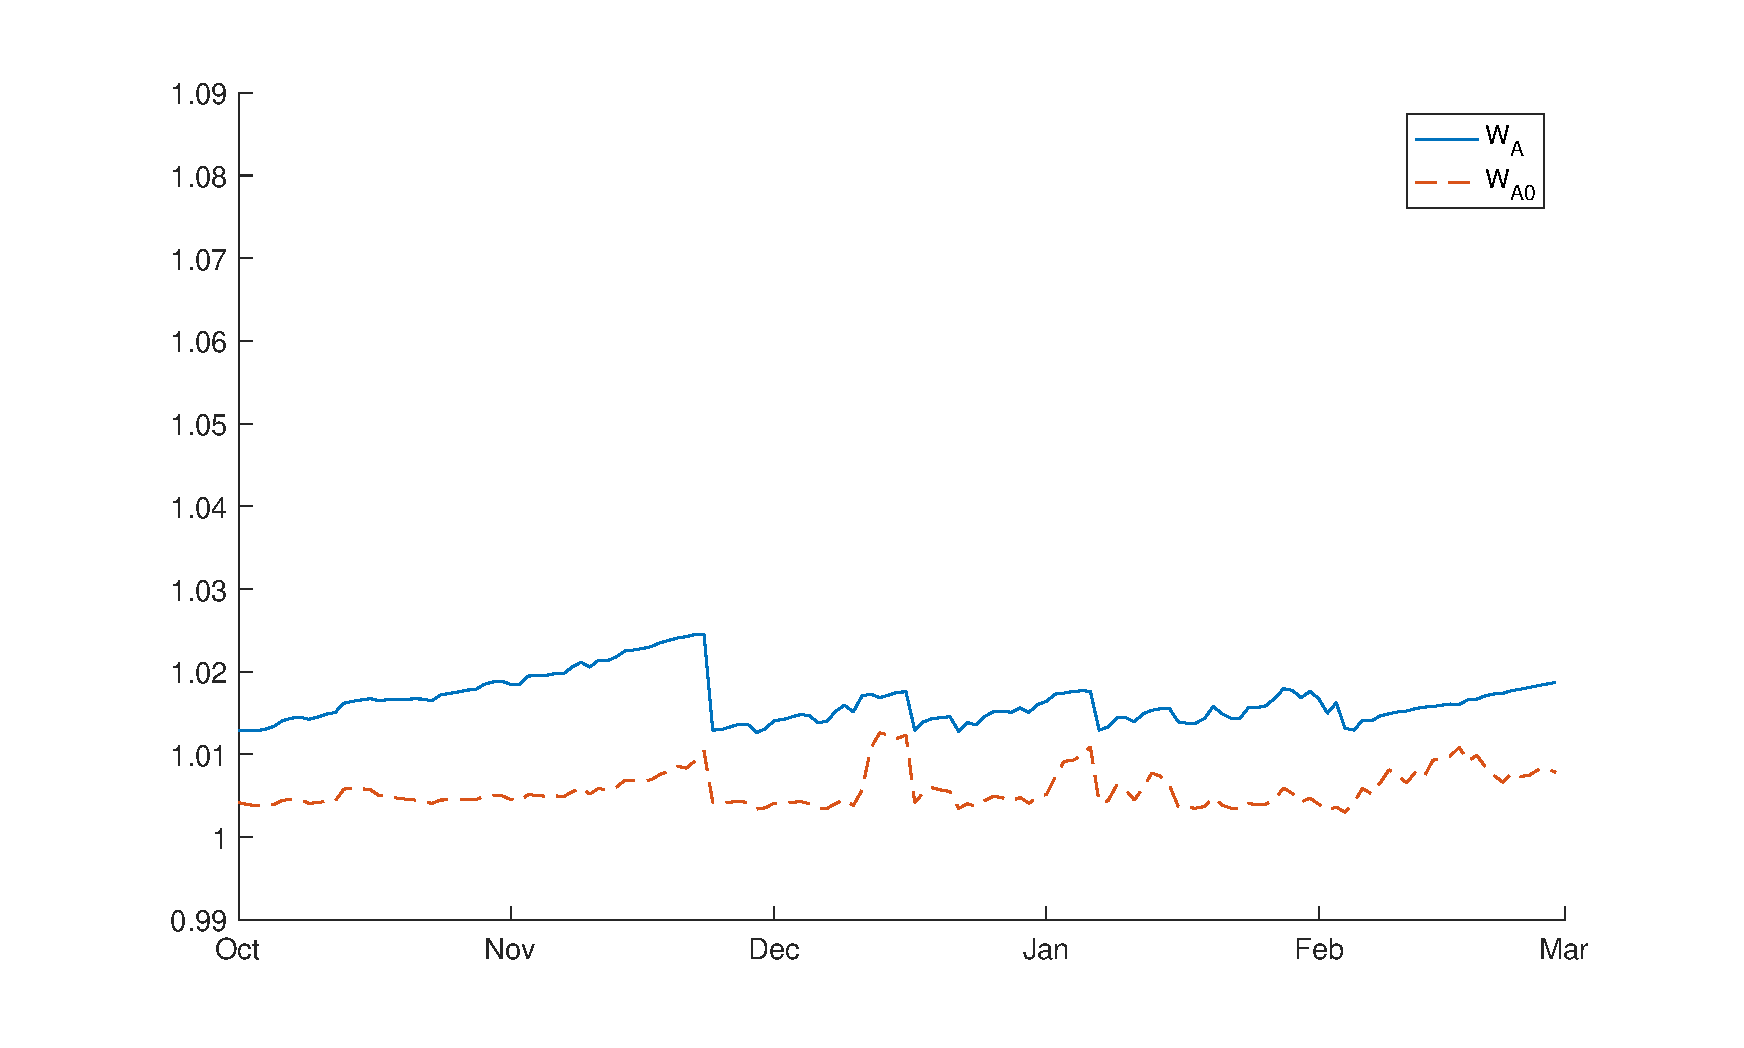
\includegraphics[width=0.95\textwidth]{WA0_alpha1.eps}
\caption{Market Value of Class A0 compared to Class A for $\alpha=1$. Annualized volatility of Class A0 is 0.0253. Parameters: $R=0.02\%,\mathcal{H}_{d}=0.25,\mathcal{H}_{u} =2,\mathcal{H}_{p}=1.02,N=100,\alpha=1$.}
\end{figure}

Class A0 token can be made even more stable by setting a high $\alpha$. Doing so results in a lower leverage ratio for Class B token, but also means a lower risk for Class A and Class A0, therefore their values will be less sensitive to the volatility of the underlying token. The following figure illustrates this with $\alpha=2$.
\begin{figure}[H]
\centering
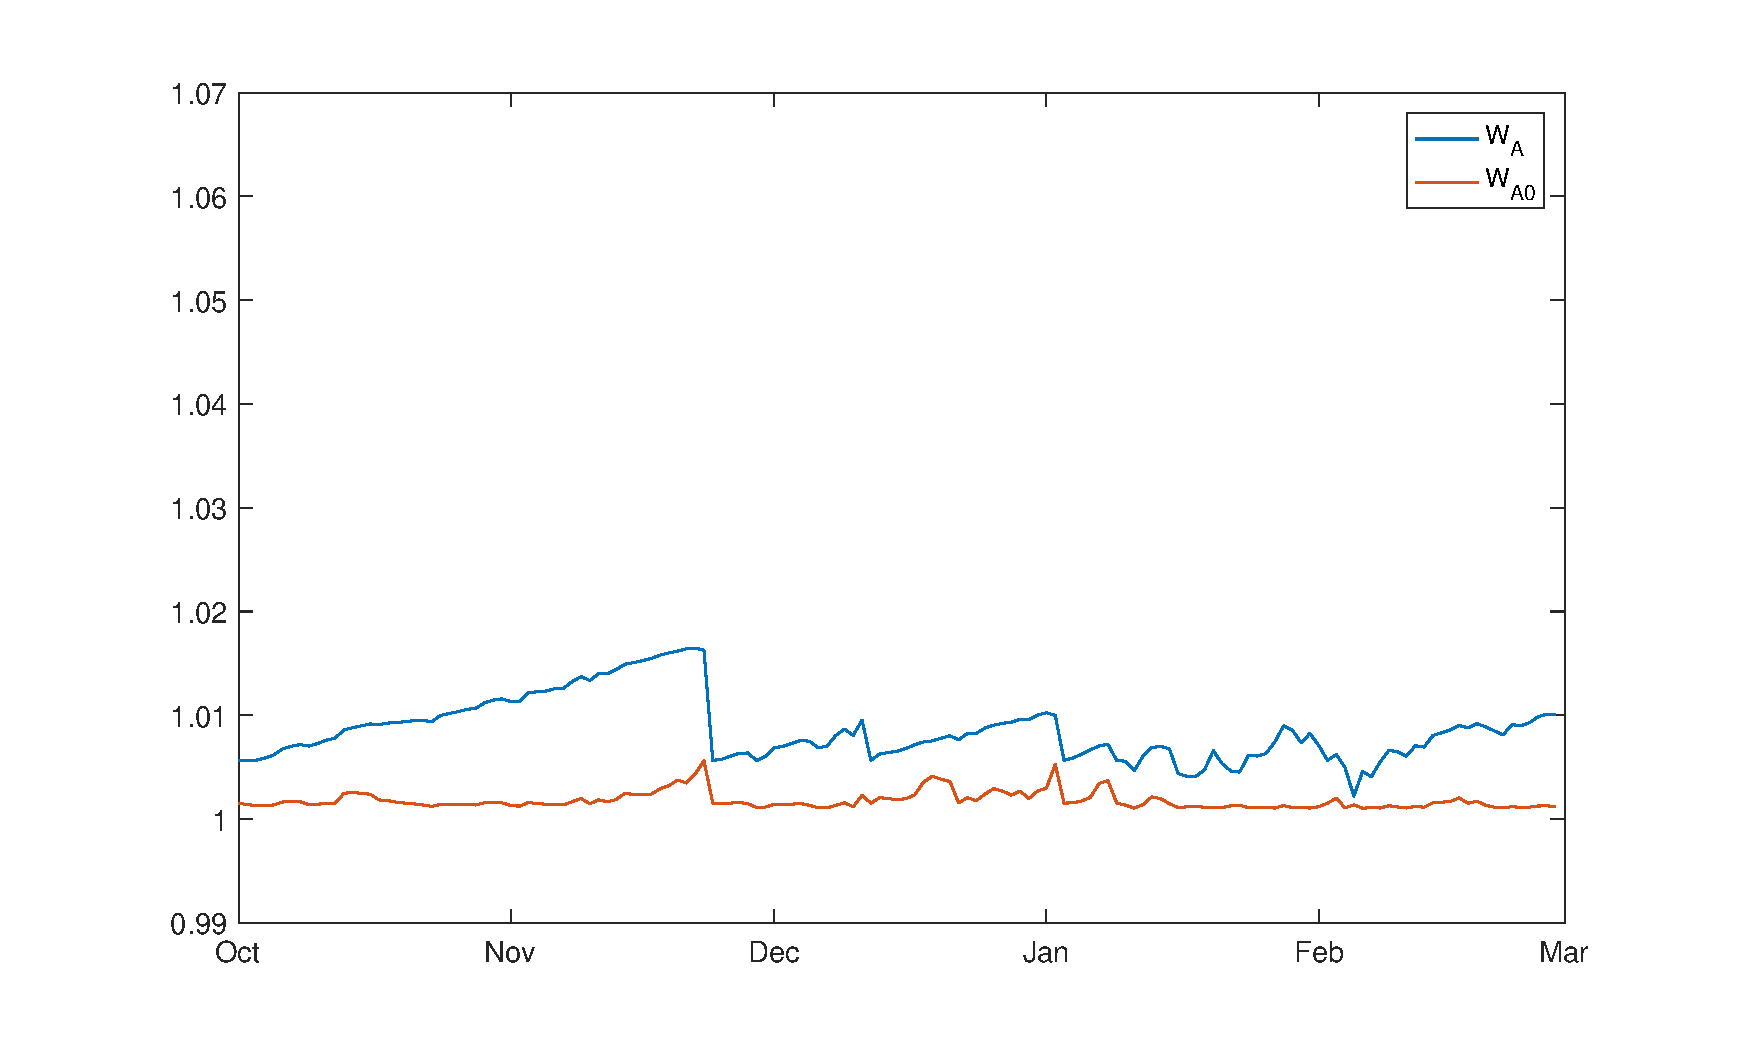
\includegraphics[width=0.95\textwidth]{WA0_alpha2.eps}
\caption{Market Value of Class A0 compared to Class A for $\alpha=2$. Annualized volatility is 0.0125. Parameters: $R=0.02\%,\mathcal{H}_{d}=0.25,\mathcal{H}_{u} =2,\mathcal{H}_{p}=1.02,N=100,\alpha=2$.}
\end{figure}

\subsection{Market Value of Class A\texorpdfstring{$^\prime$}{Lg} and B\texorpdfstring{$^\prime$}{Lg}}

\begin{figure}[H]
\centering
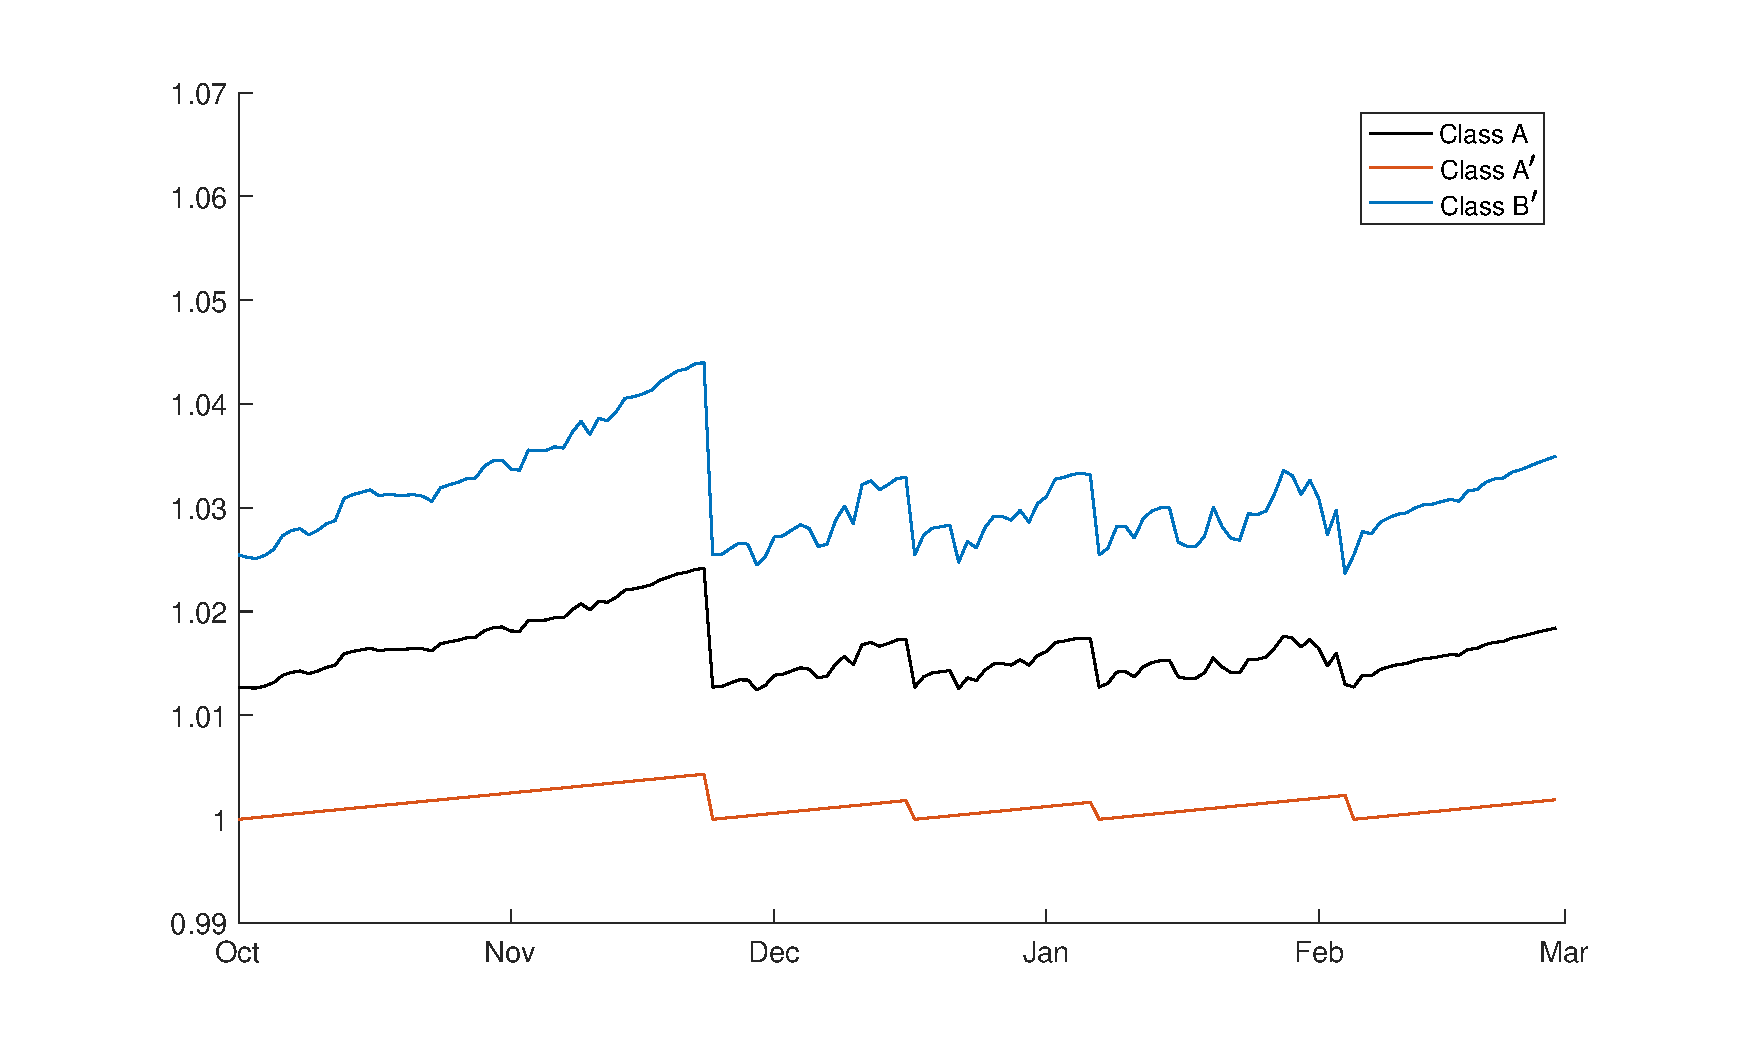
\includegraphics[width=0.95\textwidth]{WABpnoCI4.eps}
\caption{Market Value of Class A$^\prime$ (red) and B$^\prime$ (blue), compared with Class A (black). Annualized volatility of Class A$^\prime$ and B$^\prime$ are 0.0087 and 0.0397, respectively. Parameters: $R=0.02\%,\mathcal{H}_{d}=0.25,\mathcal{H}_{u} =2,\mathcal{H}_{p}=1.02,R^\prime = 0.0082\%$ ($3\%$ p.a.), $N=100, \alpha=1$.}
\end{figure}

We can see that the market value of Class A$^\prime$ token is very stable during our sample period, with a value close to 1, except for four downward jumps. These downward jumps correspond to the coupon payment of Class \Ap on the reset dates of Class A. If we de-trend the value of Class A$^\prime$ by its NAV and consider $W_{A^\prime}-V_{A^\prime}$, it has an annualized standard deviation of $5.4\times 10^{-5}$, which is much smaller than that of $W_{A}-V_{A}$ (0.0175).


\clearpage

\section{Further Development}
% \begin{flushright}
% {\small{}Patience, persistence and perspiration make an unbeatable
% combination for success.}\\
% {\small{}\textendash{} }\emph{\small{}Napoleon Hill}
% \par\end{flushright}{\small \par}

This paper has outlined the main design and market mechanism for the dual-class token structure. Further studies can be done in below aspects.

\subsubsection*{Underlying Price Pair}

While the dual class structure is independent of the underlying crypto fiat price pair, the liquidity and popularity of the underlying price pair do impact the viability of the structure as market arbitrage is important to ensure the structure trades as designed. In this paper, ETH/USD is used as the underlying price pair, but other popular ERC20 tokens, such as EOS, ADA, paired with major fiat other than USD, can also be considered.

\subsubsection*{Base Rate Discovery}

Arbitrary rate can be used for Class A coupon and it will be traded on premium or at discount based on the market required rate of return. However, it is desirable that Class A trades close to its net value, which means the coupon rate for Class A should be chosen close to the market rate. Currently there are few observable proxies in the market. Several centralized exchanges allowing margin trading are charging USD borrow rates in the range of 20\% to 40\% per annum.

As discussed in Section \ref{subsec:Premium-and-Discount}, the market premium or discount of Class A token may imply USD's borrow rate in this market. As the structure gains attractions, its implied rate could serve as an indication for other USD borrow practice in crypto market.

\subsubsection*{Optimal Reset Thresholds}

It is important to keep leverage for Class B within certain range: not too high so as to protect Class A holders from sudden price drop and not too low so as to keep Class B attractive to leveraged users. However, it is undesirable that resets, especially downward resets, happen too frequently.

There are two main parameters to be determined, the ratio between Class A and Class B shares, $\alpha$ (see Appendix \ref{subsec:General-Product-Design}); and the lower limit of Class B net value, $\mathcal{H}_{d}$ , that triggers downward resets. The Chinese market over the years has concluded a broadly accepted set of parameters: $\alpha$ is set to 1, meaning the quantities of Class A versus Class B is 1:1; $\mathcal{H}_{d}$ being 0.25, meaning a downward reset will be triggered if the underlying price dropped approximately 37.5\% from last reset. This setup has been tested in extreme market events such as the mid-2015 market crash and the early-2016 circuit breaker turmoil, where the reset clauses were all successfully implemented and protected the interests of Class A holders.

We witness that cryptocurrencies have considerably higher volatility than stock market indices. A series of back testings and Monte Carlo simulations will be performed to investigate the optimal parameters for dual class token structures.

\clearpage

\begin{appendices}

\section{General Product Design}\label{subsec:General-Product-Design}

% \subsection{General Product Design\label{subsec:General-Product-Design}}

In Section \ref{sec:Product-Design}, we have described a specific product design where Class A is stable relative to USD as target fiat currency and Class B has initial leverage as 2. In addition, transaction cost in creation and redemption is omitted. In this section, a general case is discussed.

\subsection{Creation}

Dual-class tokens can be created by depositing underlying tokens to the Custodian contract. Upon receiving underlying tokens of amount $M_{C}$, the Custodian contract will return to the sender certain amount of Class A and Class B tokens. Such amount $C_{A}$ and $C_{B}$ can be calculated by:
\begin{equation}
\begin{array}{cc}
C_{B}= & \frac{M_{C}\cdot P_{0}\cdot\left(1-c\right)}{1+\alpha}\\
C_{A}= & C_{B}\cdot\alpha\ ,
\end{array}\label{eq:creation-1}
\end{equation}
where $c$ is the processing fee of the smart contract, $\alpha$ is a positive number to determine the ratio of A and B, and $P_{0}$ is the recorded price of underlying token in target fiat currency at last reset event.

\subsection{Redemption}

Holders of Class A and Class B tokens can withdraw deposited underlying tokens at any time by performing a redemption. To do this, the user will send amount of $C\cdot\alpha$ Class A and amount of $C$ Class B tokens to the Custodian contract. The contract will deduct Class A and Class B tokens, and return to the sender $M_{C}$ underlying tokens, where $M_{C}$ can be calculated by:
\begin{equation}
M_{C}=\frac{C\cdot\left(1-c\right)\cdot\left(1+\alpha\right)}{P_{0}}\ .\label{eq:redemption-1}
\end{equation}

\subsection{Net Value}

The net value of tokens are calculated based on the coupon rate, the elapsed time from last reset event, and the latest underlying token price in target fiat currency fed to the system. In particular:
\begin{equation}
\begin{array}{cc}
V_{A}^{t}= & 1+R\cdot t\\
V_{B}^{t}= & \left(1+\alpha\right)\cdot\frac{P_{t}}{P_{0}}-\alpha\cdot V_{A}^{t}\ ,
\end{array}\label{eq:netvalue-1}
\end{equation}
where $R$ is the daily coupon rate, $t$ is the number of days from last reset event, and $P_{t}$ is the current price of underlying token in target fiat currency.

\subsection{Quantity}

Below holds in the system at all time
\[
Q_{A}^{t}=Q_{B}^{t}\cdot\alpha\ ,
\]
where $Q_{A}^{t}$ and $Q_{B}^{t}$ are the total amount of Class A and Class B tokens.

\subsection{Implied Leverage Ratio}

\begin{align*}
L_{B}^{t} & =\frac{P_{t}}{P_{0}}\cdot\frac{\left(1+\alpha\right)}{V_{B}^{t}}
\end{align*}
Note that at inception or after resets, above simply reduces to $L_{B}^{0}=1+\alpha$.

\subsection{Contingent Upward Reset\label{subsec:Contingent-Upward-Reset}}

An upward reset is triggered when $V_{B}^{t}\geqslant\mathcal{H}_{u}$. Upon upward reset:
\begin{enumerate}
\item Total amount of both classes token remain unchanged, $Q_{A}^{t+}=Q_{A}^{t-}$ and $Q_{B}^{t+}=Q_{B}^{t-}$.
\item Net Value of both classes reset to 1 target fiat currency.
\item Both classes' holders will receive certain amount of underlying token
from the Custodian contract. Such amount for each Class A token is
$U_{A}=\frac{V_{A}^{t-}-1}{P_{t}}$ and for each Class B token is
$U_{B}=\frac{V_{B}^{t-}-1}{P_{t}}$.
\end{enumerate}
Total value in the system is unchanged after reset:
\begin{align*}
 & U_{A}\cdot P_{t}\cdot Q_{A}^{t-}+U_{B}\cdot P_{t}\cdot Q_{B}^{t-}+Q_{A}^{t+}\cdot V_{A}^{t+}+Q_{B}^{t+}\cdot V_{B}^{t+}\\
= & \left(V_{A}^{t-}-1\right)\cdot Q_{A}^{t-}+\left(V_{B}^{t-}-1\right)\cdot Q_{B}^{t-}+Q_{A}^{t-}\cdot1+Q_{B}^{t-}\cdot1\\
= & V_{A}^{t-}\cdot Q_{A}^{t-}+V_{B}^{t-}\cdot Q_{B}^{t-}\ .
\end{align*}

\subsection{Contingent Downward Reset\label{subsec:Contingent-Downward-Reset}}

A downward reset is triggered when $V_{B}^{t}\leqslant\mathcal{H}_{d}$. Upon downward reset:
\begin{enumerate}
\item Total amount of Class B token is reduced to $Q_{B}^{t+}=Q_{B}^{t-}\cdot V_{B}^{t-}$.
\item Total amount of Class A token is reduced to $Q_{A}^{t+}=Q_{B}^{t+}\cdot\alpha$.
\item Net Value of both classes reset to 1 target fiat currency.
\item Class A holders will receive certain amount of underlying token from the Custodian contract. Such amount of each Class A token is: $D_{A}=\frac{V_{A}^{t-}-V_{B}^{t-}}{P_{t}}$.
\end{enumerate}
Total value in the system is unchanged after reset:
\begin{align*}
 & D_{A}\cdot P_{t}\cdot Q_{A}^{t-}+Q_{A}^{t+}\cdot V_{A}^{t+}+Q_{B}^{t+}\cdot V_{B}^{t+}\\
= & \left(V_{A}^{t-}-V_{B}^{t-}\right)\cdot Q_{A}^{t-}+Q_{B}^{t+}\cdot\alpha\cdot1+Q_{B}^{t+}\cdot1\\
= & V_{A}^{t-}\cdot Q_{A}^{t-}-V_{B}^{t-}\cdot Q_{B}^{t-}\cdot\alpha+Q_{B}^{t-}\cdot V_{B}^{t-}\cdot\alpha+Q_{B}^{t-}\cdot V_{B}^{t-}\\
= & V_{A}^{t-}\cdot Q_{A}^{t-}+V_{B}^{t-}\cdot Q_{B}^{t-}\ .
\end{align*}
Note above used the fact $Q_{A}^{t-}=Q_{B}^{t-}\cdot\alpha$.

\subsection{Periodic Reset}

A periodic reset is triggered when $V_{A}^{t}\geqslant\mathcal{H}_{p}$. If $V_{B}^{t-}$ is less than 1, reset will be the same as the Contingent Downward reset. Otherwise, reset will be the same as the Contingent Upward reset.

\section{General Market Arbitrage}

The price parity shall hold as below:
\[
\alpha\cdot P_{A}^{t}+P_{B}^{t}=\alpha\cdot V_{A}^{t}+V_{B}^{t}\ ,
\]
where $P_{A}^{t}$ is the current price of Class A in target fiat currency, and $P_{B}^{t}$ is the current price of Class B in target fiat currency.

Along with Equation (\ref{eq:creation-1}), (\ref{eq:redemption-1}) and (\ref{eq:netvalue-1}) in Section \ref{subsec:General-Product-Design}, below should hold:
\[
\frac{P_{t}}{P_{0}}\cdot\left(1-c\right)\leq\frac{\alpha\cdot P_{A}^{t}+P_{B}^{t}}{1+\alpha}\leq\frac{P_{t}}{P_{0}}\cdot\frac{1}{1-c}\ .
\]
On open market, arbitrage opportunity exists when Class A and Class B tokens trade away from their net values and above equation is violated on either side.

\paragraph{Arbitrage via Creation}

When combined market price of Class A and Class B tokens are higher than their combined net values, i.e.
\[
\frac{\alpha\cdot P_{A}^{t}+P_{B}^{t}}{1+\alpha}>\frac{P_{t}}{P_{0}}\cdot\frac{1}{1-c}\ ,
\]
arbitrage profit can be exploited by perform DUO token creation:
\begin{enumerate}
\item Buy $\frac{1}{1-c}$ underlying tokens from open market for $P_{t}\cdot\frac{1}{1-c}$ target fiat currency equivalent.
\item Send the underlying tokens to the Custodian contract.
\item Based on Equation (\ref{eq:creation-1}), receive $P_{0}\cdot\frac{\alpha}{1+\alpha}$ Class A and $P_{0}\cdot\frac{1}{1+\alpha}$ Class B tokens.
\item Sell Class A and Class B tokens on open market for $P_{0}\cdot\frac{\alpha P_{A}^{t}+P_{B}^{t}}{1+\alpha}$ target fiat currency equivalent.
\end{enumerate}
The expected payoff of above operations is:
\[
P_{0}\cdot\frac{\alpha P_{A}^{t}+P_{B}^{t}}{1+\alpha}-\frac{P_{t}}{1-c}=P_{0}\cdot\left(\frac{\alpha\cdot P_{A}^{t}+P_{B}^{t}}{1+\alpha}-\frac{P_{t}}{P_{0}}\cdot\frac{1}{1-c}\right)>0\ .
\]

\paragraph{Arbitrage via Redemption}

When combined market price of Class A and Class B tokens are lower than their combined net values, i.e.
\[
\frac{P_{t}}{P_{0}}\cdot\left(1-c\right)>\frac{\alpha\cdot P_{A}^{t}+P_{B}^{t}}{1+\alpha}\ ,
\]
similar arbitrage profit can be exploited by perform DUO token redemption:
\begin{enumerate}
\item Buy $P_{0}\cdot\frac{\alpha}{1+\alpha}$ Class A and $P_{0}\cdot\frac{1}{1+\alpha}$ Class B tokens from open market for $P_{0}\cdot\frac{\alpha P_{A}^{t}+P_{B}^{t}}{1+\alpha}$ target fiat currency equivalent.
\item Send Class A and Class B tokens to the Custodian contract.
\item Based on Equation (\ref{eq:redemption-1}), receive $1-c$ underlying tokens.
\item Sell underlying tokens on open market for $P_{t}\cdot\left(1-c\right)$ target fiat currency equivalent.
\end{enumerate}
The expected payoff of above operations is:
\[
P_{t}\cdot\left(1-c\right)-P_{0}\cdot\frac{\alpha P_{A}^{t}+P_{B}^{t}}{1+\alpha}=P_{0}\cdot\left(\frac{P_{t}}{P_{0}}\cdot\left(1-c\right)-\frac{\alpha\cdot P_{A}^{t}+P_{B}^{t}}{1+\alpha}\right)>0\ .
\]

\section{Derivation of the Pricing Equation}
In this section we show that \eqref{VAL2} defines a unique bounded function $W_A$, which is exactly the solution to the PDE problem \eqref{eqn:PDEstart} -- \eqref{eqn:PDEend}. We denote $v_s$ and $Y_s$ as the time from last interest payment and the number of A shares at time $s$, respectively. Starting from an initial value 1, $Y$ is reduced by a factor of $\mathcal{H}_d$(resp. $1-g(S)$) on every downward (resp. periodic) reset dates, reflecting the partial payback of Class A principal. Further denote $\zeta_i$, $\tau_i$, and $\eta_i$ as the $i$-th pre-specified payment date, upward reset date, and downward reset date after $t$, respectively. From the construction of contract,
\begin{align*}
S_{\zeta_i}=S_{\tau_i}=S_{\eta_i}=1, ~~v_{\tau_i}=v_{\eta_i}=v_{\zeta_i}=0.
\end{align*}

\begin{thm}\label{thm:main}
$W_{A}$ is the unique classical solution\footnote{By classical solution we mean $W_{A}\in C^{1,2}(Q)\cap C(\overline{Q}\backslash D)$, where $Q=\{(t,S):0\le t<1,H_{d}(t)<S<H_{u}(t)\}$ and $D=\{T\}\times\{H_{d}(T),H_{u}(T)\}$.} to the following partial differential equation on $\{(t,S):0\le t<T,H_{d}(t)<S<H_{u}(t)\}$
\begin{align}
-\frac{\partial W_{A}}{\partial t} & =\frac{1}{2}\sigma^{2}S^{2}\frac{\partial^{2}W_{A}}{\partial S^{2}}+r S\frac{\partial W_{A}}{\partial S}-r W_{A}\\
W_{A}(T,S) & =RT+g(S)+(1-g(S))W_{A}(0,1)\\
W_{A}(t,H_{u}(t)) & =Rt+W_{A}(0,1)\\
W_{A}(t,H_d(t)) & =Rt+1-\mathcal{H}_{d}+\mathcal{H}_{d}W_{A}(0,1).
\end{align}
\end{thm}

\begin{proof}[Proof of Theorem \ref{thm:main}]
	Using Theorem E1.1 in \cite{DM2018}, we can rewrite \eqref{VAL2} in a non-recursive form as
	\begin{align}\label{VALnonrecur}
	\begin{split}
	W_A(t,S)&=E_t^{(t,S,1)}\Bigg[\sum_{\zeta_i\ge t}e^{-R(\zeta_i-t)}Y_{\zeta_i-}(RT+g(S_{\zeta-}))+\sum_{\tau_i\ge t}e^{-R(\tau_i-t)}Y_{\tau_i-}rv_{\tau_i-}\\
	&\quad+\sum_{\eta_i\ge t}e^{-R(\eta_i-t)}Y_{\eta_i-}(rv_{\eta_i-}+1-\mathcal{H}_d)\Bigg],
	\end{split}
	\end{align}
	where $E^{(u,s,y)}_t$ is the $\mathbb{Q}$-expectation computed under the initial condition $v_{t-}=u$, $S_{t-}=s$, and $Y_{t-}=y$. Following the proof in Section 4.1 in \cite{Dai:2016vj} shows that \eqref{VALnonrecur} is the unique classical solution to the PDE problem \eqref{eqn:PDEstart} -- \eqref{eqn:PDEend}. Therefore, $W_A$ defined in \eqref{VAL2} is the unique classical solution to \eqref{eqn:PDEstart} -- \eqref{eqn:PDEend}.
\end{proof}

\section{Numerical Procedure for the Pricing Equation \texorpdfstring{\eqref{eqn:PDEstart} -- \eqref{eqn:PDEend}}{Lg}}\label{subsec:Numerical-Procedure-for}

We propose an iterative algorithm to obtain a numerical solution of the periodic parabolic terminal-boundary value problem ($\ref{eqn:PDEstart}$) \textendash{} ($\ref{eqn:PDEend}$).

\subsection*{Algorithm 1}
\begin{enumerate}
\item \textit{Set the initial guess $W_{A}^{(0)}=0$; }
\item \textit{For $i=1,2,\cdots$: Given $W_{A}^{(i-1)}$, solve for $W_{A}^{(i)}$, the solution to the equation
\begin{align*}
-\frac{\partial W_{A}}{\partial t}= & \frac{1}{2}\sigma^{2}S^{2}\frac{\partial^{2}W_{A}}{\partial S^{2}}+r S\frac{\partial W_{A}}{\partial S}-r W_{A} &  & 0\le t<T,H_{d}(t)<S<H_{u}(t)\\
W_{A}(1,S)= & RT+g(S)+(1-g(S))W_{A}^{(i-1)}(0,1) &  & H_{d}(t)<S<H_{u}(t)\\
W_{A}(t,H_{u}(t))= & Rt+W_{A}^{(i-1)}(0,1) &  & 0\le t\le T\\
W_{A}(t,H_{d}(t))= & Rt+1-\mathcal{H}_{d}+\mathcal{H}_{d}W_{A}^{(i-1)}(0,1) &  & 0\le t\le T.
\end{align*}
}
\item \textit{If $||W_{A}^{(i)}-W_{A}^{(i-1)}||<$ tolerance, stop and return $W_{A}^{(i)}$; otherwise set $i=i+1$ and go to step 2. }
\end{enumerate}
By using a similar proof as Theorem C.1 in \cite{DM2018}, one can show that the sequence $(W_{A}^{(i)})_{i\ge1}$ defined in Algorithm 1 is monotonically increasing and converges to $W_{A}$ uniformly.

\end{appendices}

\section*{\clearpage{}}
\begin{thebibliography}{1}

\bibitem[1]{AC}Adams, A. T., and J. B. Clunie. 2006. Risk Assessment Techniques for Split Capital Investment Trusts. \textit{Annals of Actuarial Science} 1:7-36.


\bibitem[2]{DM2018}Dai, M., S. Kou, C. Yang, and Z. Ye. 2018. The Overpricing of Leveraged Products: A Case Study of Dual-Purpose Funds in China. \textit{Working Paper}.

\bibitem[3]{Dai:2016vj}Dai, M., S. Kou, and C. Yang. 2017. A Stochastic Representation for Nonlocal Parabolic PDEs with Applications. \textit{Working Paper}.


\bibitem[4]{Ingersoll1976}Ingersoll, J. E. 1976. A Theoretical and Empirical Investigation of the Dual Purpose Funds: an Application of Contingent-claims Analysis. \textit{Journal of Financial Economics} 3:83-123.

\bibitem[5]{JO}Jarrow, R. A., and M. O'Hara. 1989. Primes and Scores: An Essay on Market Imperfections. \textit{The Journal of Finance} 44:1263-1287.

\bibitem[6]{BS}Black, F., and M. Scholes. 1973. The Pricing of Options and Corporate Liabilities. \textit{Journal of Political Economy} 81:637-654.

\bibitem[7]{Leverage}Leverage. \textit{\href{https://www.investopedia.com/terms/l/leverage.asp}{https://www.investopedia.com/terms/l/leverage.asp}}

\bibitem[8]{ETH}White Paper: A Next-Generation Smart Contract and Decentralized Application Platform. \textit{\href{https://github.com/ethereum/wiki/wiki/White-Paper}{https://github.com/ethereum/wiki/wiki/White-Paper}}

\bibitem[9]{USDT}Tether: Fiat currencies on the Bitcoin blockchain. \textit{\href{https://tether.to/wp-content/uploads/2016/06/TetherWhitePaper.pdf}{https://tether.to/wp-content/uploads/2016/06/TetherWhitePaper.pdf}}

\bibitem[10]{Basecoin}Basecoin: A Price-Stable Cryptocurrency with an Algorithmic Central Bank. \textit{\href{http://www.getbasecoin.com/basecoin_whitepaper_0_99.pdf}{http://www.getbasecoin.com/basecoin\_{}whitepaper\_{}0\_{}99.pdf}}

\bibitem[11]{MAKERDAO}The Dai Stablecoin System. \textit{\href{https://makerdao.com/whitepaper/DaiDec17WP.pdf}{https://makerdao.com/whitepaper/DaiDec17WP.pdf}}
\end{thebibliography}

\end{document}
